\documentclass[notitlepage,letterpaper,12pt]{article} % para articulo

% Este es un comentario <- Los comentarios comienzan con % 
% todo lo que se escriba hasta el final de la linea será ignorado <- Este es otro comentario

%Lenguaje del documento
\usepackage[spanish]{babel} % silabea palabras castellanas <- Puedo poner comentarios para explicar de que va este comando en la misma línea

%Encoding
\usepackage[utf8]{inputenc} % Acepta caracteres en castellano
\usepackage[T1]{fontenc} % Encoding de salida al pdf

%Paquetes mara mayor comodidad
\usepackage[normalem]{ulem}
\providecommand{\e}[1]{\ensuremath{\times 10^{#1}}}
\usepackage{aas_macros}

\usepackage{textcomp}
\usepackage{gensymb}


%Hipertexto
\usepackage[colorlinks=true,urlcolor=blue,linkcolor=blue]{hyperref} % navega por el doc: hipertexto y links

%Aquello de las urls
\usepackage{url} 

%simbolos matemáticos
\usepackage{amsmath}
\usepackage{amsfonts}
\usepackage{amssymb}
\usepackage{physics} 

% permite insertar gráficos, imágenes y figuras, en pdf o en eps
\usepackage{graphicx}
\usepackage{epstopdf}
\usepackage{multirow}
\usepackage{float}
\usepackage[export]{adjustbox}
% geometría del documento, encabezados y pies de páginas, márgenes
\usepackage{geometry}
\usepackage{comment}
\geometry{letterpaper}       % ... o a4paper o a5paper o ... 

\usepackage{quotmark}
\usepackage{natbib}


\usepackage{fancyhdr} % encabezados y pies de pg
\pagestyle{fancy}
\chead{\bfseries {}}
\lhead{} % si se omite coloca el nombre de la seccion
%\rhead{fecha del doc}
\lfoot{\it Informe Semana 8.}
\cfoot{ }
\rfoot{Universidad de los Andes}
%\rfoot{\thepage}
%margenes
\voffset = -0.25in
\textheight = 8.0in
\textwidth = 6.5in
\oddsidemargin = 0.in
\headheight = 20pt
\headwidth = 6.5in
\renewcommand{\headrulewidth}{0.5pt}
\renewcommand{\footrulewidth}{0,5pt}

\begin{document}
\title{Informe para Jaime: semana 8}
\author{
\textbf{Javier Alejandro Acevedo Barroso\thanks{e-mail: \texttt{ja.acevedo12@uniandes.edu.co}}}\\
\textit{Universidad de los Andes, Bogotá, Colombia}\\
} % Hasta aquí llega el bloque "author" (son dos autores por informe, orden alfabético)

%\date{Versión $\alpha \beta$ fecha del documento}
\maketitle %Genera el título del documento


%Resumen

%\begin{abstract}

%Usando un generador de señales 	CFG253 como fuente de voltaje en el circuito requerido de la practica, se observo la señal que produce un circuito RLC en un osciloscopio, con el objetivo de estudiar su resonancia eléctrica mediante la curva generada a partir de graficar el voltaje en la resistencia vs la frecuencia de oscilacion dada por la fuente  


 
%\end{abstract}

%Introducción
\section{Objetivos semanales}
\begin{enumerate}
\item Probar a 1024 mi código con inestabilidad usando solver de \citet{FUKA2015356}.
\item Probar inestabilidad de Jeans para Mocz variando resolución (disminuir hasta una resolución mínima de 32).
\end{enumerate}

\section{Corriendo el código de Mocz (2016)}
El principal problema con usar el código de \citet{integerLatticeDynamics} es la dependencia con el código de Vladimir Fuka para resolver la ecuación de Poisson.
Para instalar \tqt{PoisFFT} (el solver de Fuka) se usa Scons.
El script de configuración para scons es \tqt{srs/Sconstruct}, para instalar en Linux usando los compiladores de GNU se debe comentar la línea 137 del archivo Sconstruct.
En caso de que cambie el código fuente, la línea a comentar es: \tqt{env.Append(FORTRANMODDIRPREFIX = '-J')}.
Una vez corregido, se puede instalar sin problema PoisFFT siguiendo las instrucciones del README, lo mismo para el código de Mocz.




El código de Mocz está disponible en \url{https://github.com/pmocz/IntegerLattice}

El solver de V.Fuka está disponible en \url{https://github.com/LadaF/PoisFFT}.
Guardaré una copia del código fuente para la eternidad, en caso de que deje se estar en Github.

\section{Correr mi código a 1024 con solver}
Corrí mi código usando el solver de Fuka a 1024 para la inestabilidad de Jeans y funciona a la perfección. Definitivamente hacer un solver perfecto es complicado.

A continuación presento la evolución temporal a 1024:

\begin{figure}[h]
  \centering
   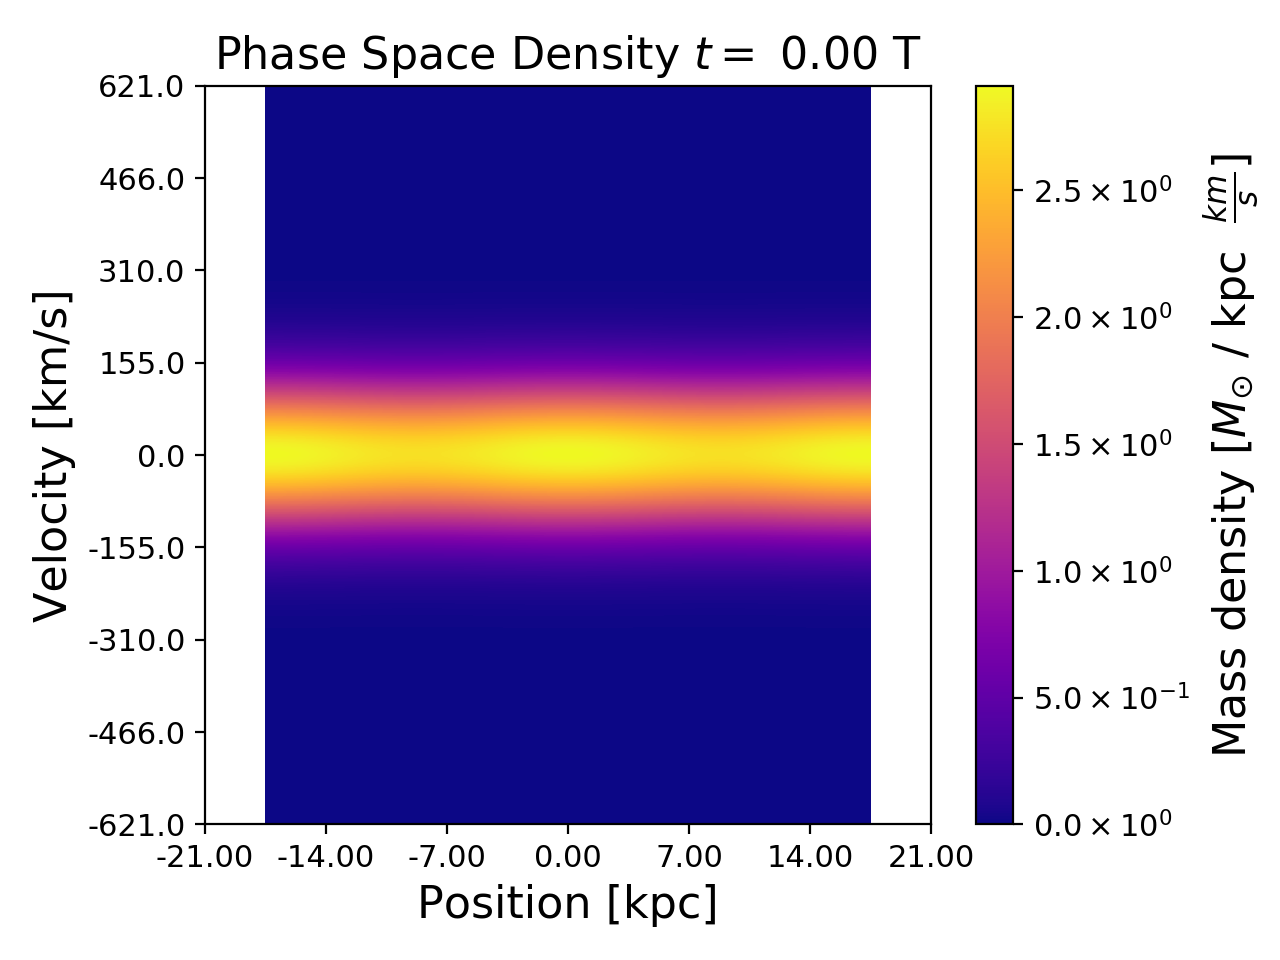
\includegraphics[scale= 0.5]{y1024phase0.png}
      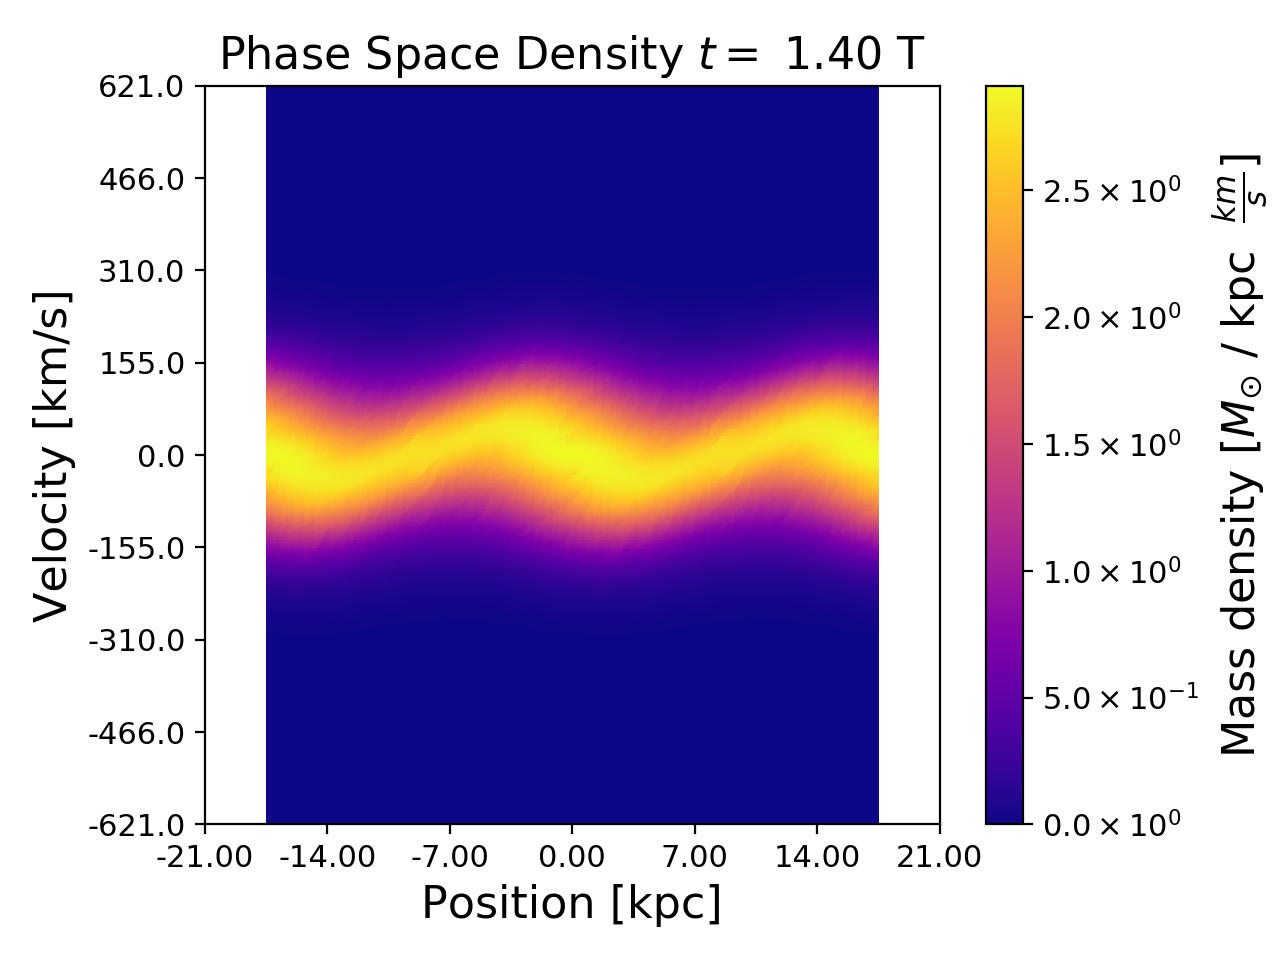
\includegraphics[scale= 0.5]{y1024phase14.png}
         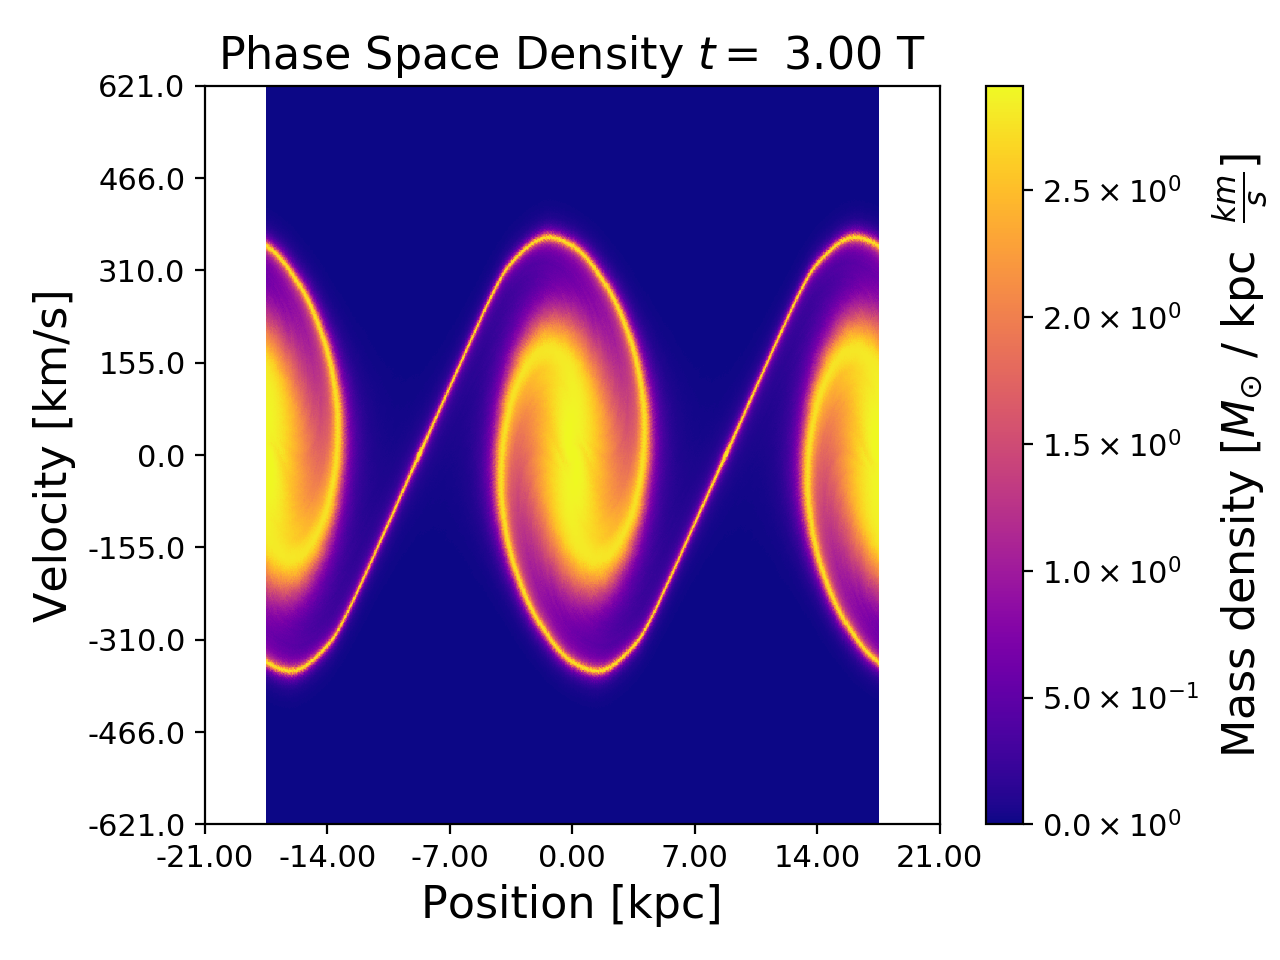
\includegraphics[scale= 0.5]{y1024phase30.png}
            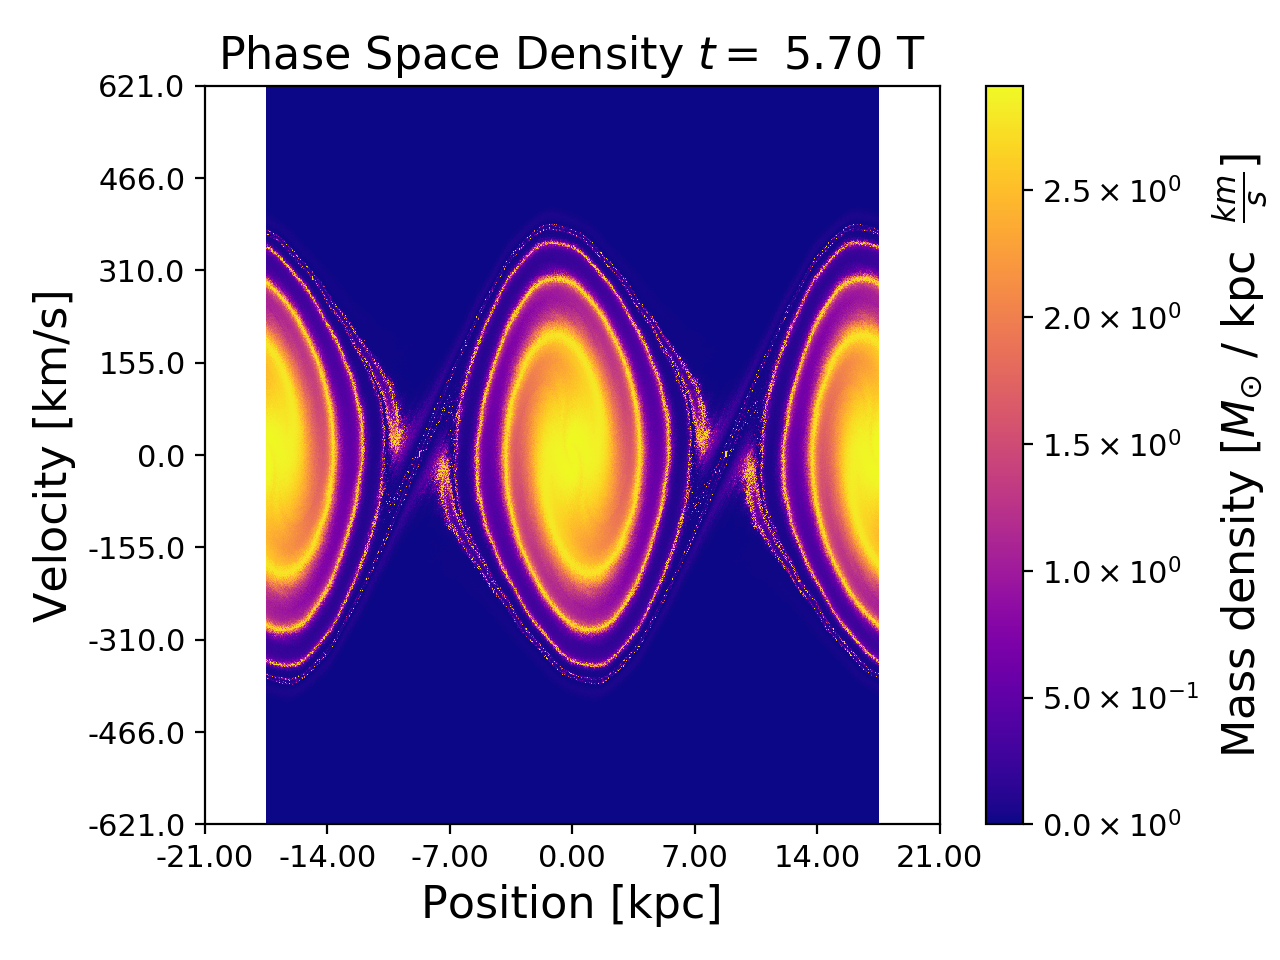
\includegraphics[scale= 0.5]{y1024phase57.png}
%  \caption{ asd}
  \label{fig: cobre}
\end{figure}	

También probé para 512, infortunadamente no se activa la inestabilidad de Jeans.


\section{Conservación de energía para Mocz}
Corrí la inestabilidad de Jeans con las mismas condiciones con las que corrí la mía en la sección anterior ($k/k_j = 0.5$) para diferentes resoluciones.
Para N menor que 512 falla la inestabilidad de Jeans.
Para N mayor a 512 se activa la inestabilidad de Jeans con una evolución temporal de energía idéntica.
Para N igual a 512 se activa la inestabilidad de Jeans pero la evolución temporal es ligeramente diferente a las otras resoluciones que también activan la inestabilidad.

A continuación presento la evolución temporal del a energía para los casos en los que no se activa la inestabilidad de Jeans.

\begin{figure}[h]
  \centering
   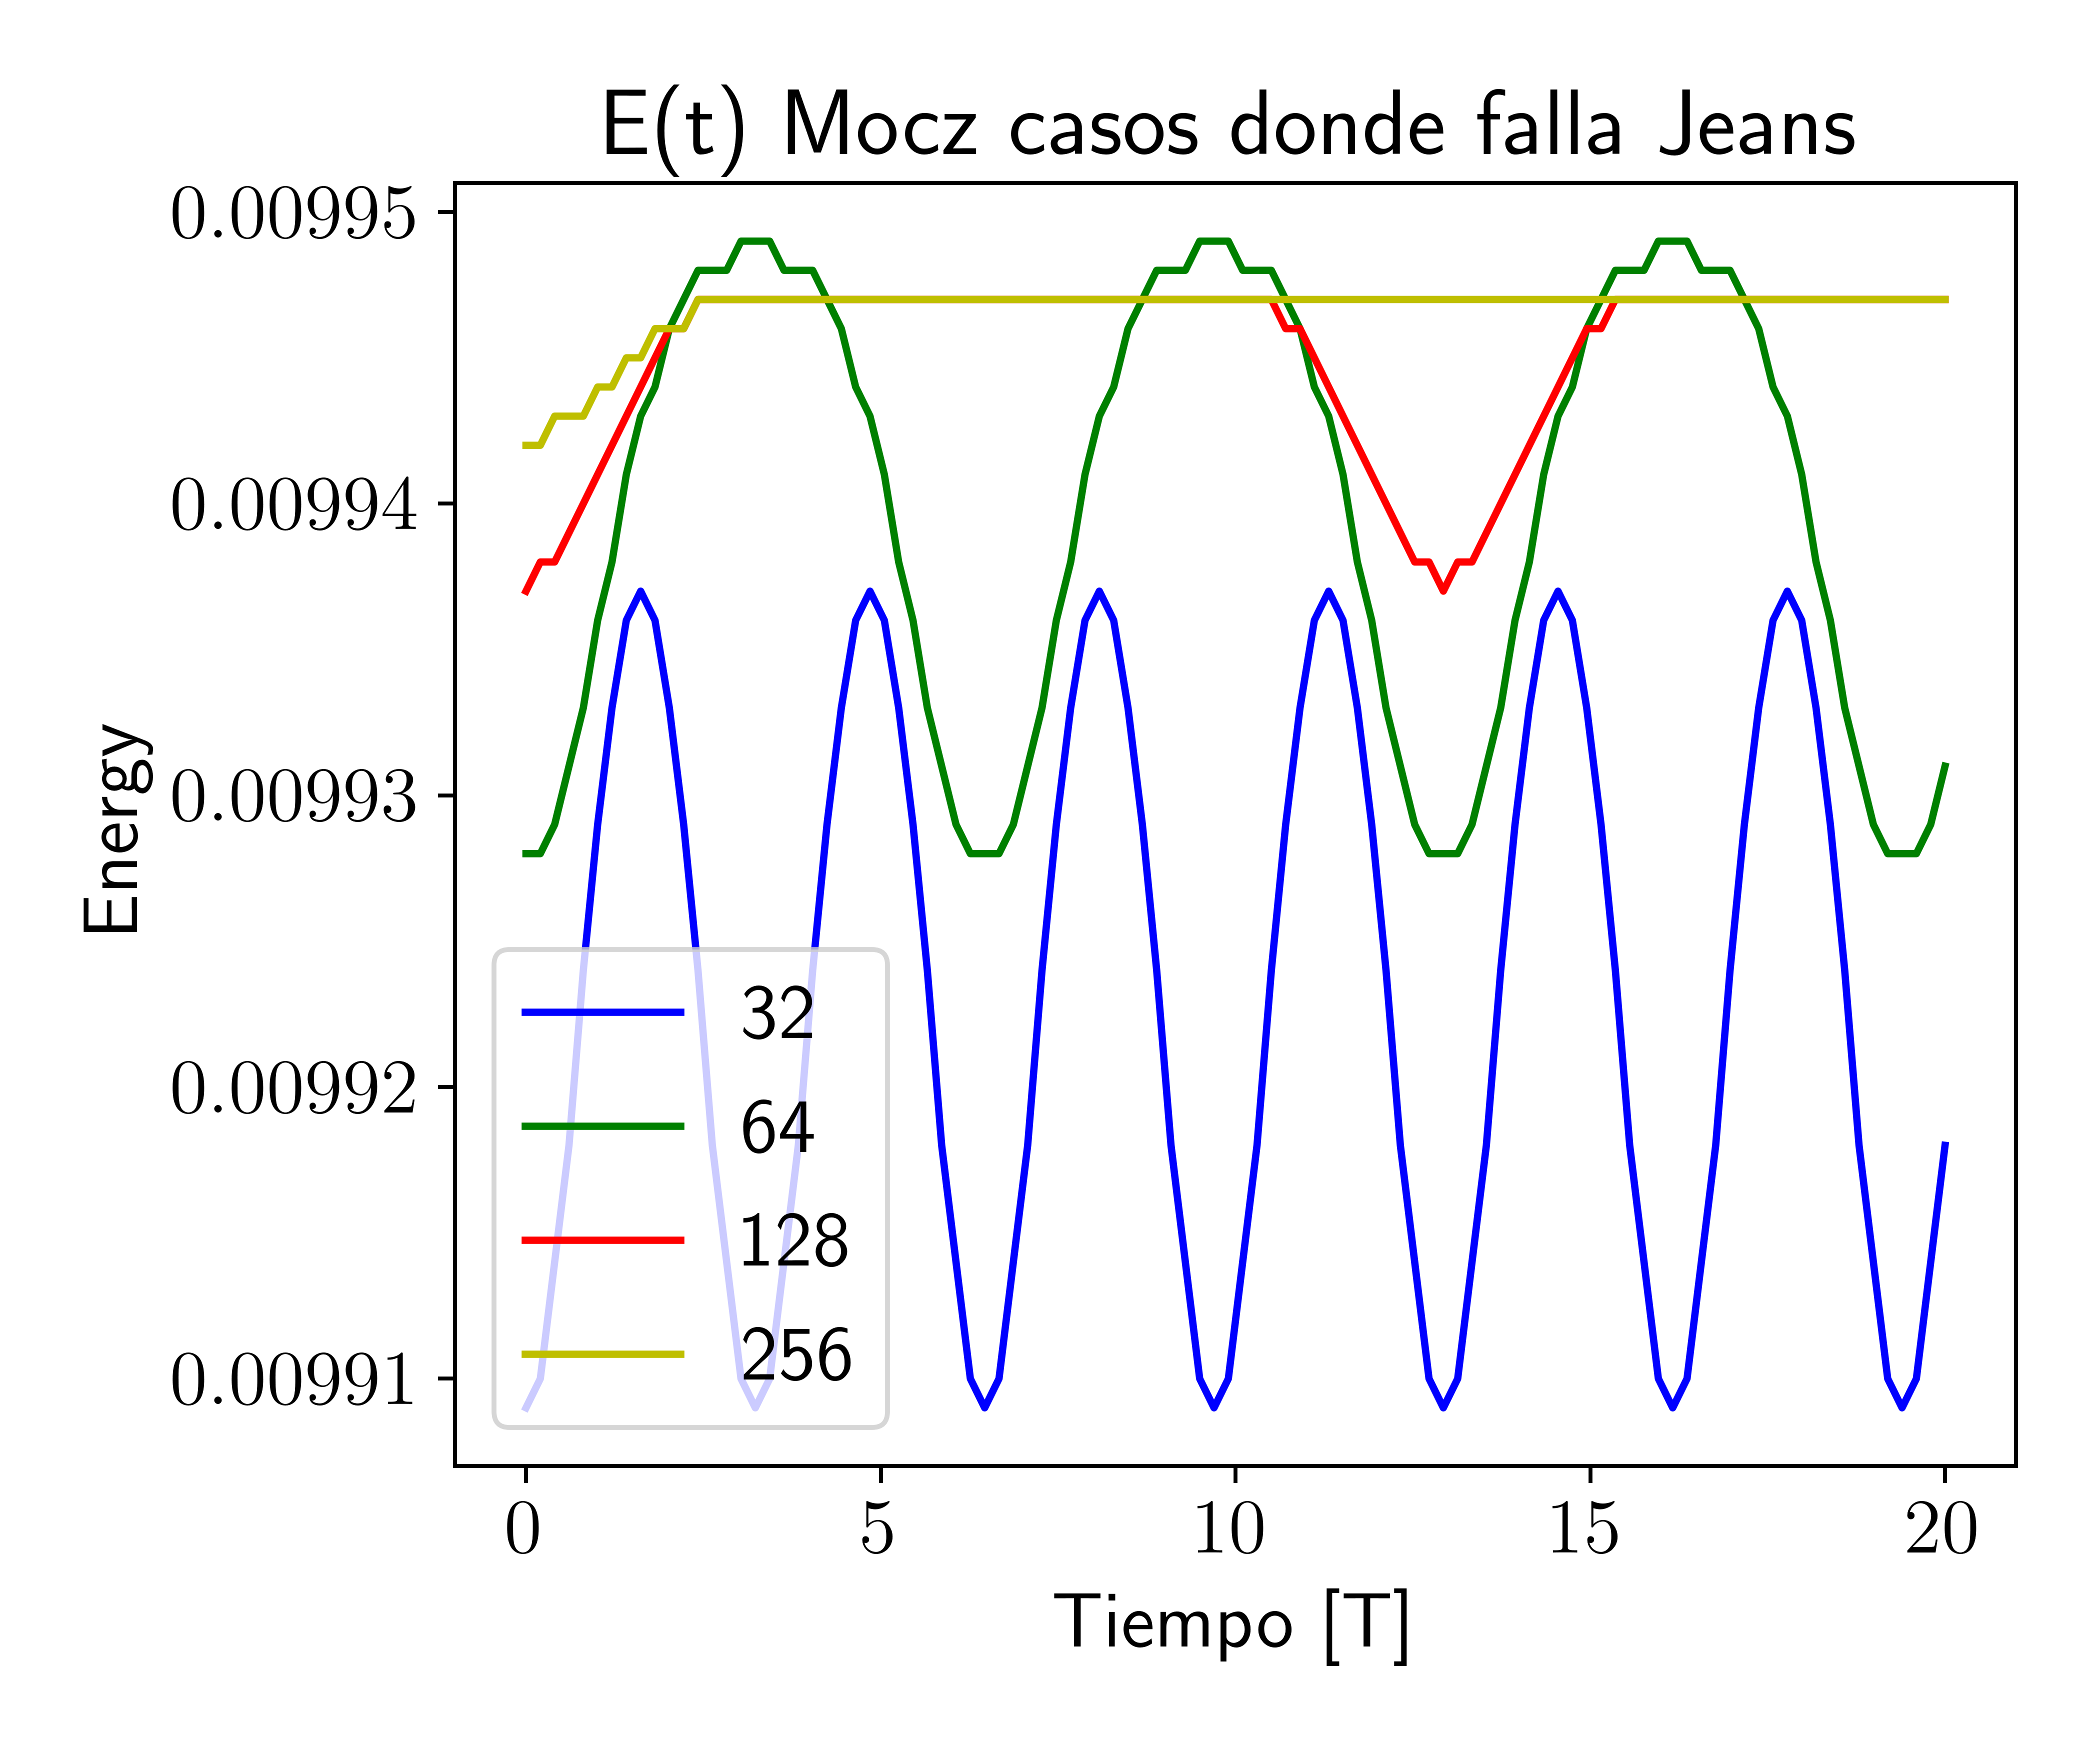
\includegraphics[scale= 0.6]{JeansFails.png}
%  \caption{ asd}
  \label{fig: cobre}
\end{figure}	

Se observa que no se sobreponen las curvas pero que en general son variaciones pequeñas.
\newpage

A continuación la gráfica para los casos en los que se activa la inestabilidad de Jeans.


\begin{figure}[h]
  \centering
   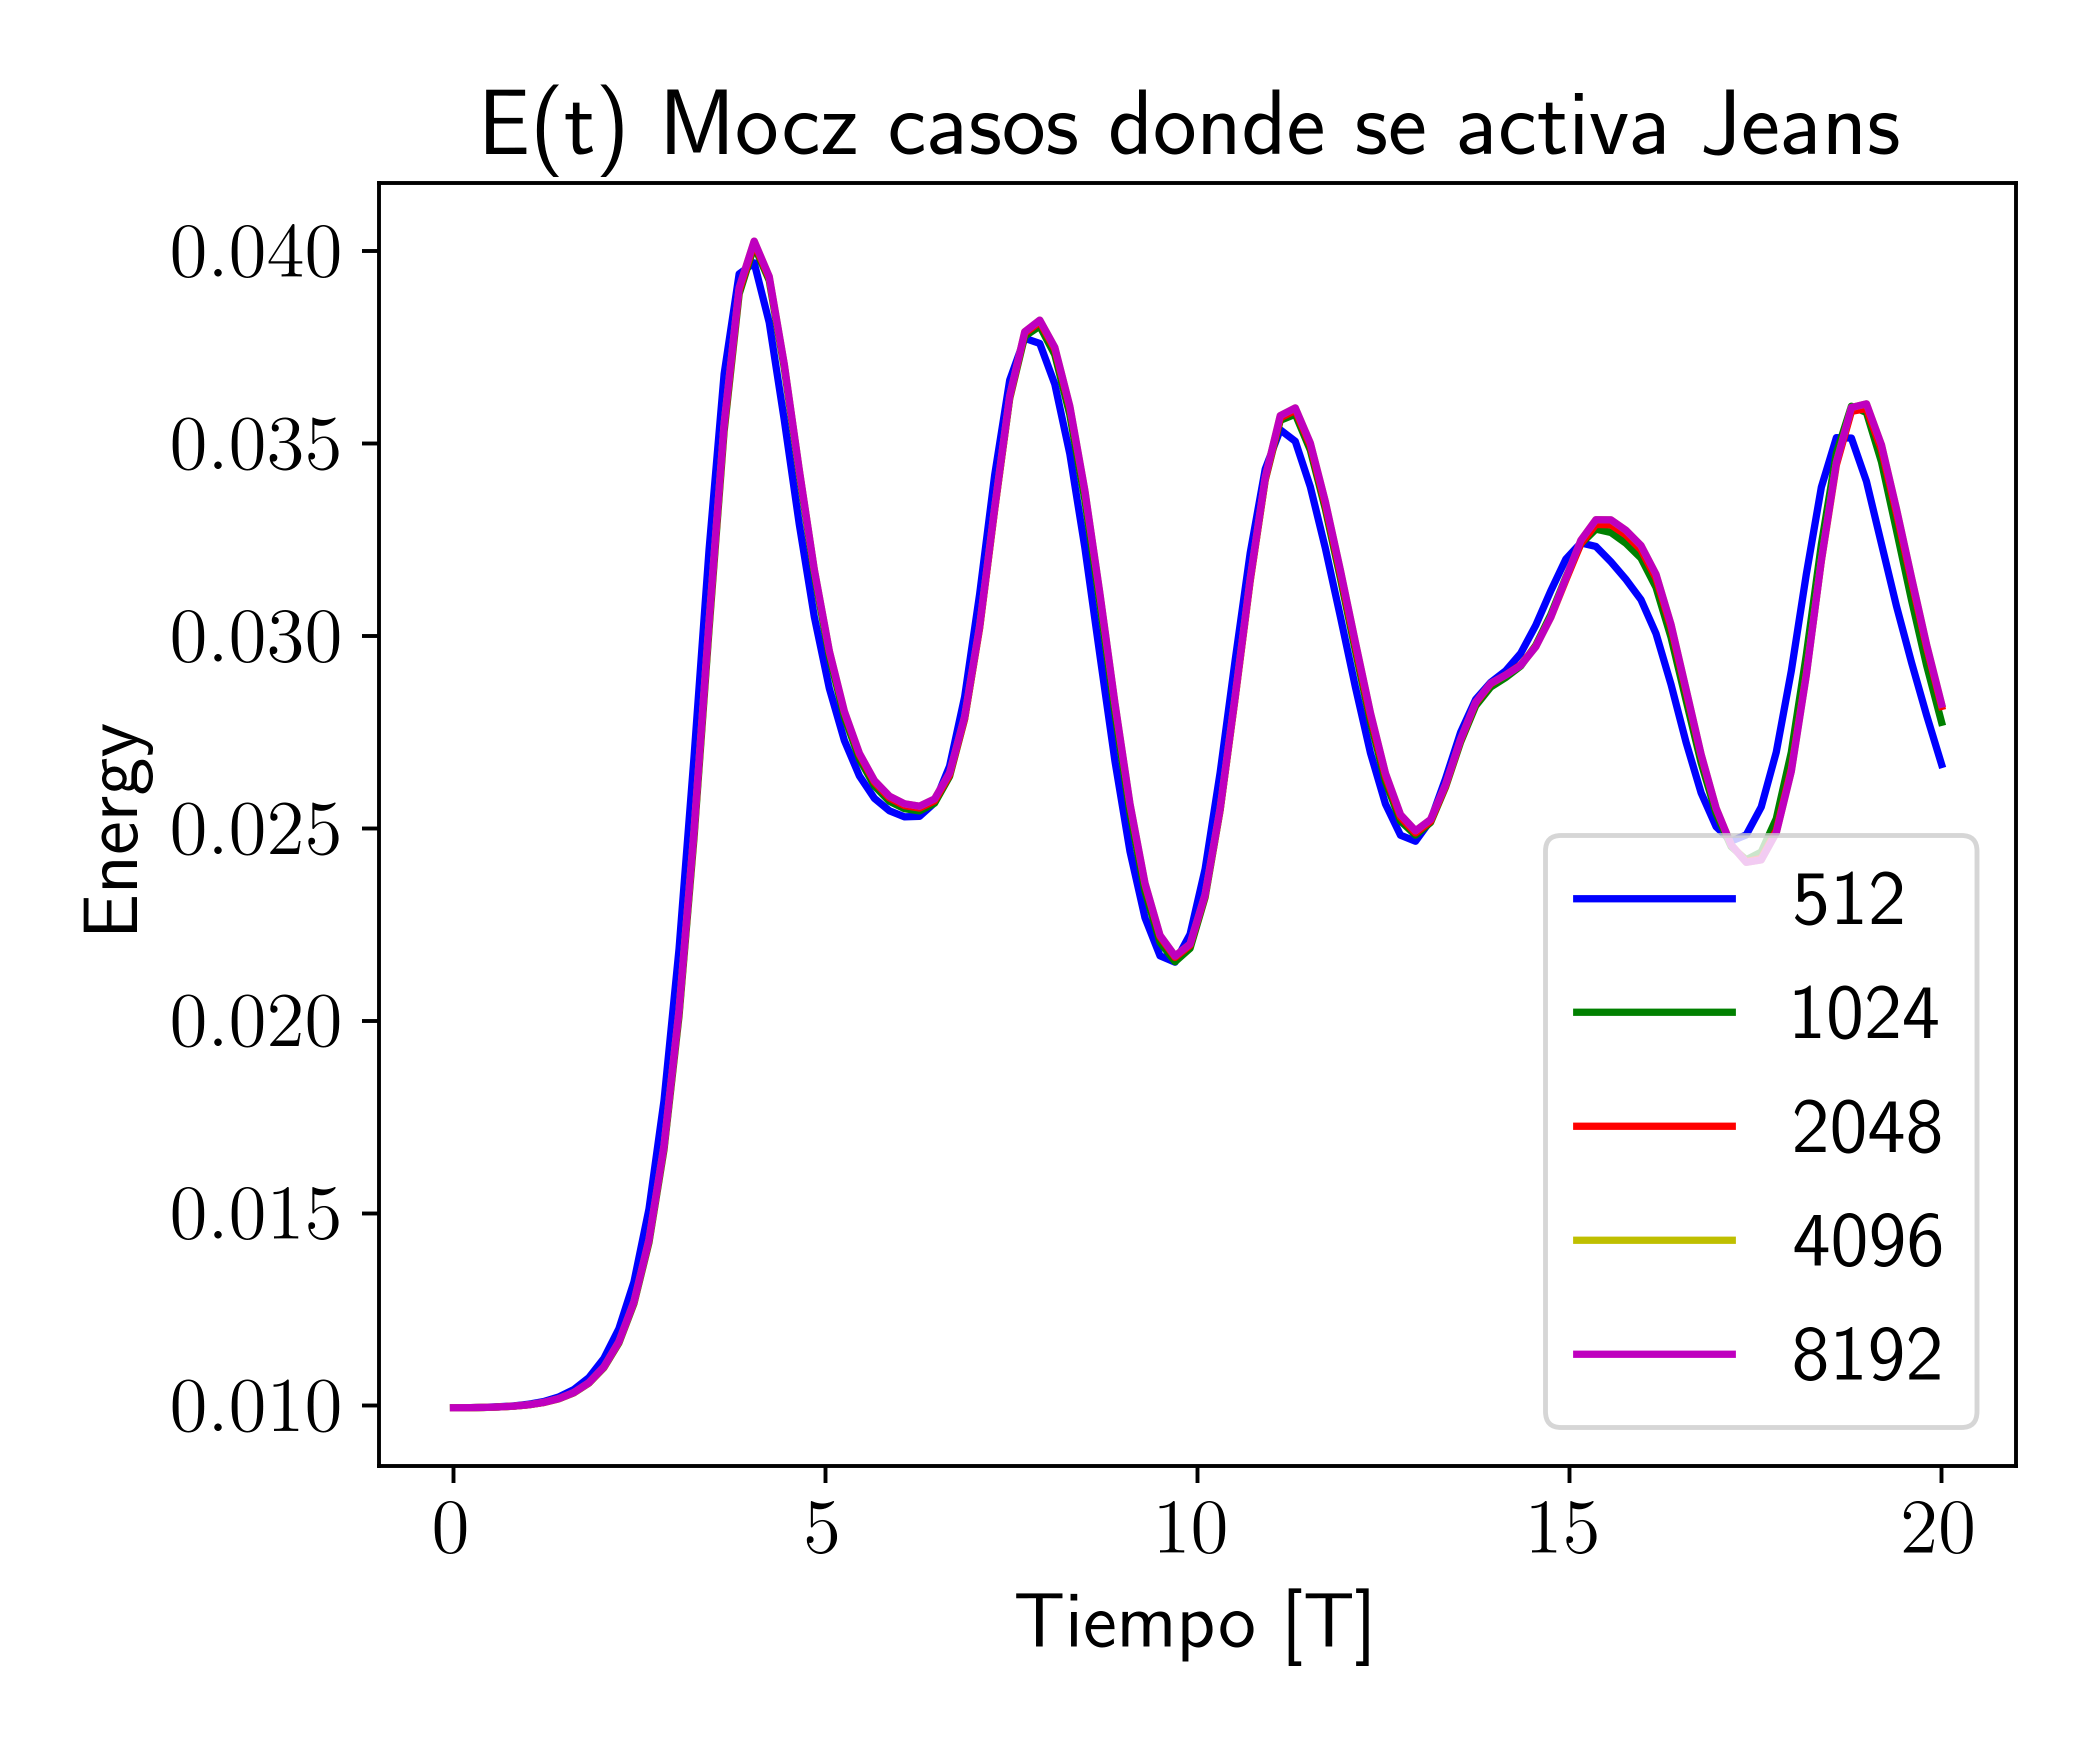
\includegraphics[scale= 0.6]{JeansActivates.png}
%  \caption{ asd}
  \label{fig: cobre}
\end{figure}	

El caso de N = 512 es el único que se separa. Los demás son completamente idénticos entre sí.

Se observa a demás que el código de Mocz logra activar la inestabilidad a 512 mientras que el mío solo llega hasta 1024. Sin embargo la evolución energética parece indicar que no termina de converger a esa resolución.






\newpage
Por último, incluyo como lucen todas las curvas juntas

\begin{figure}[h]
  \centering
   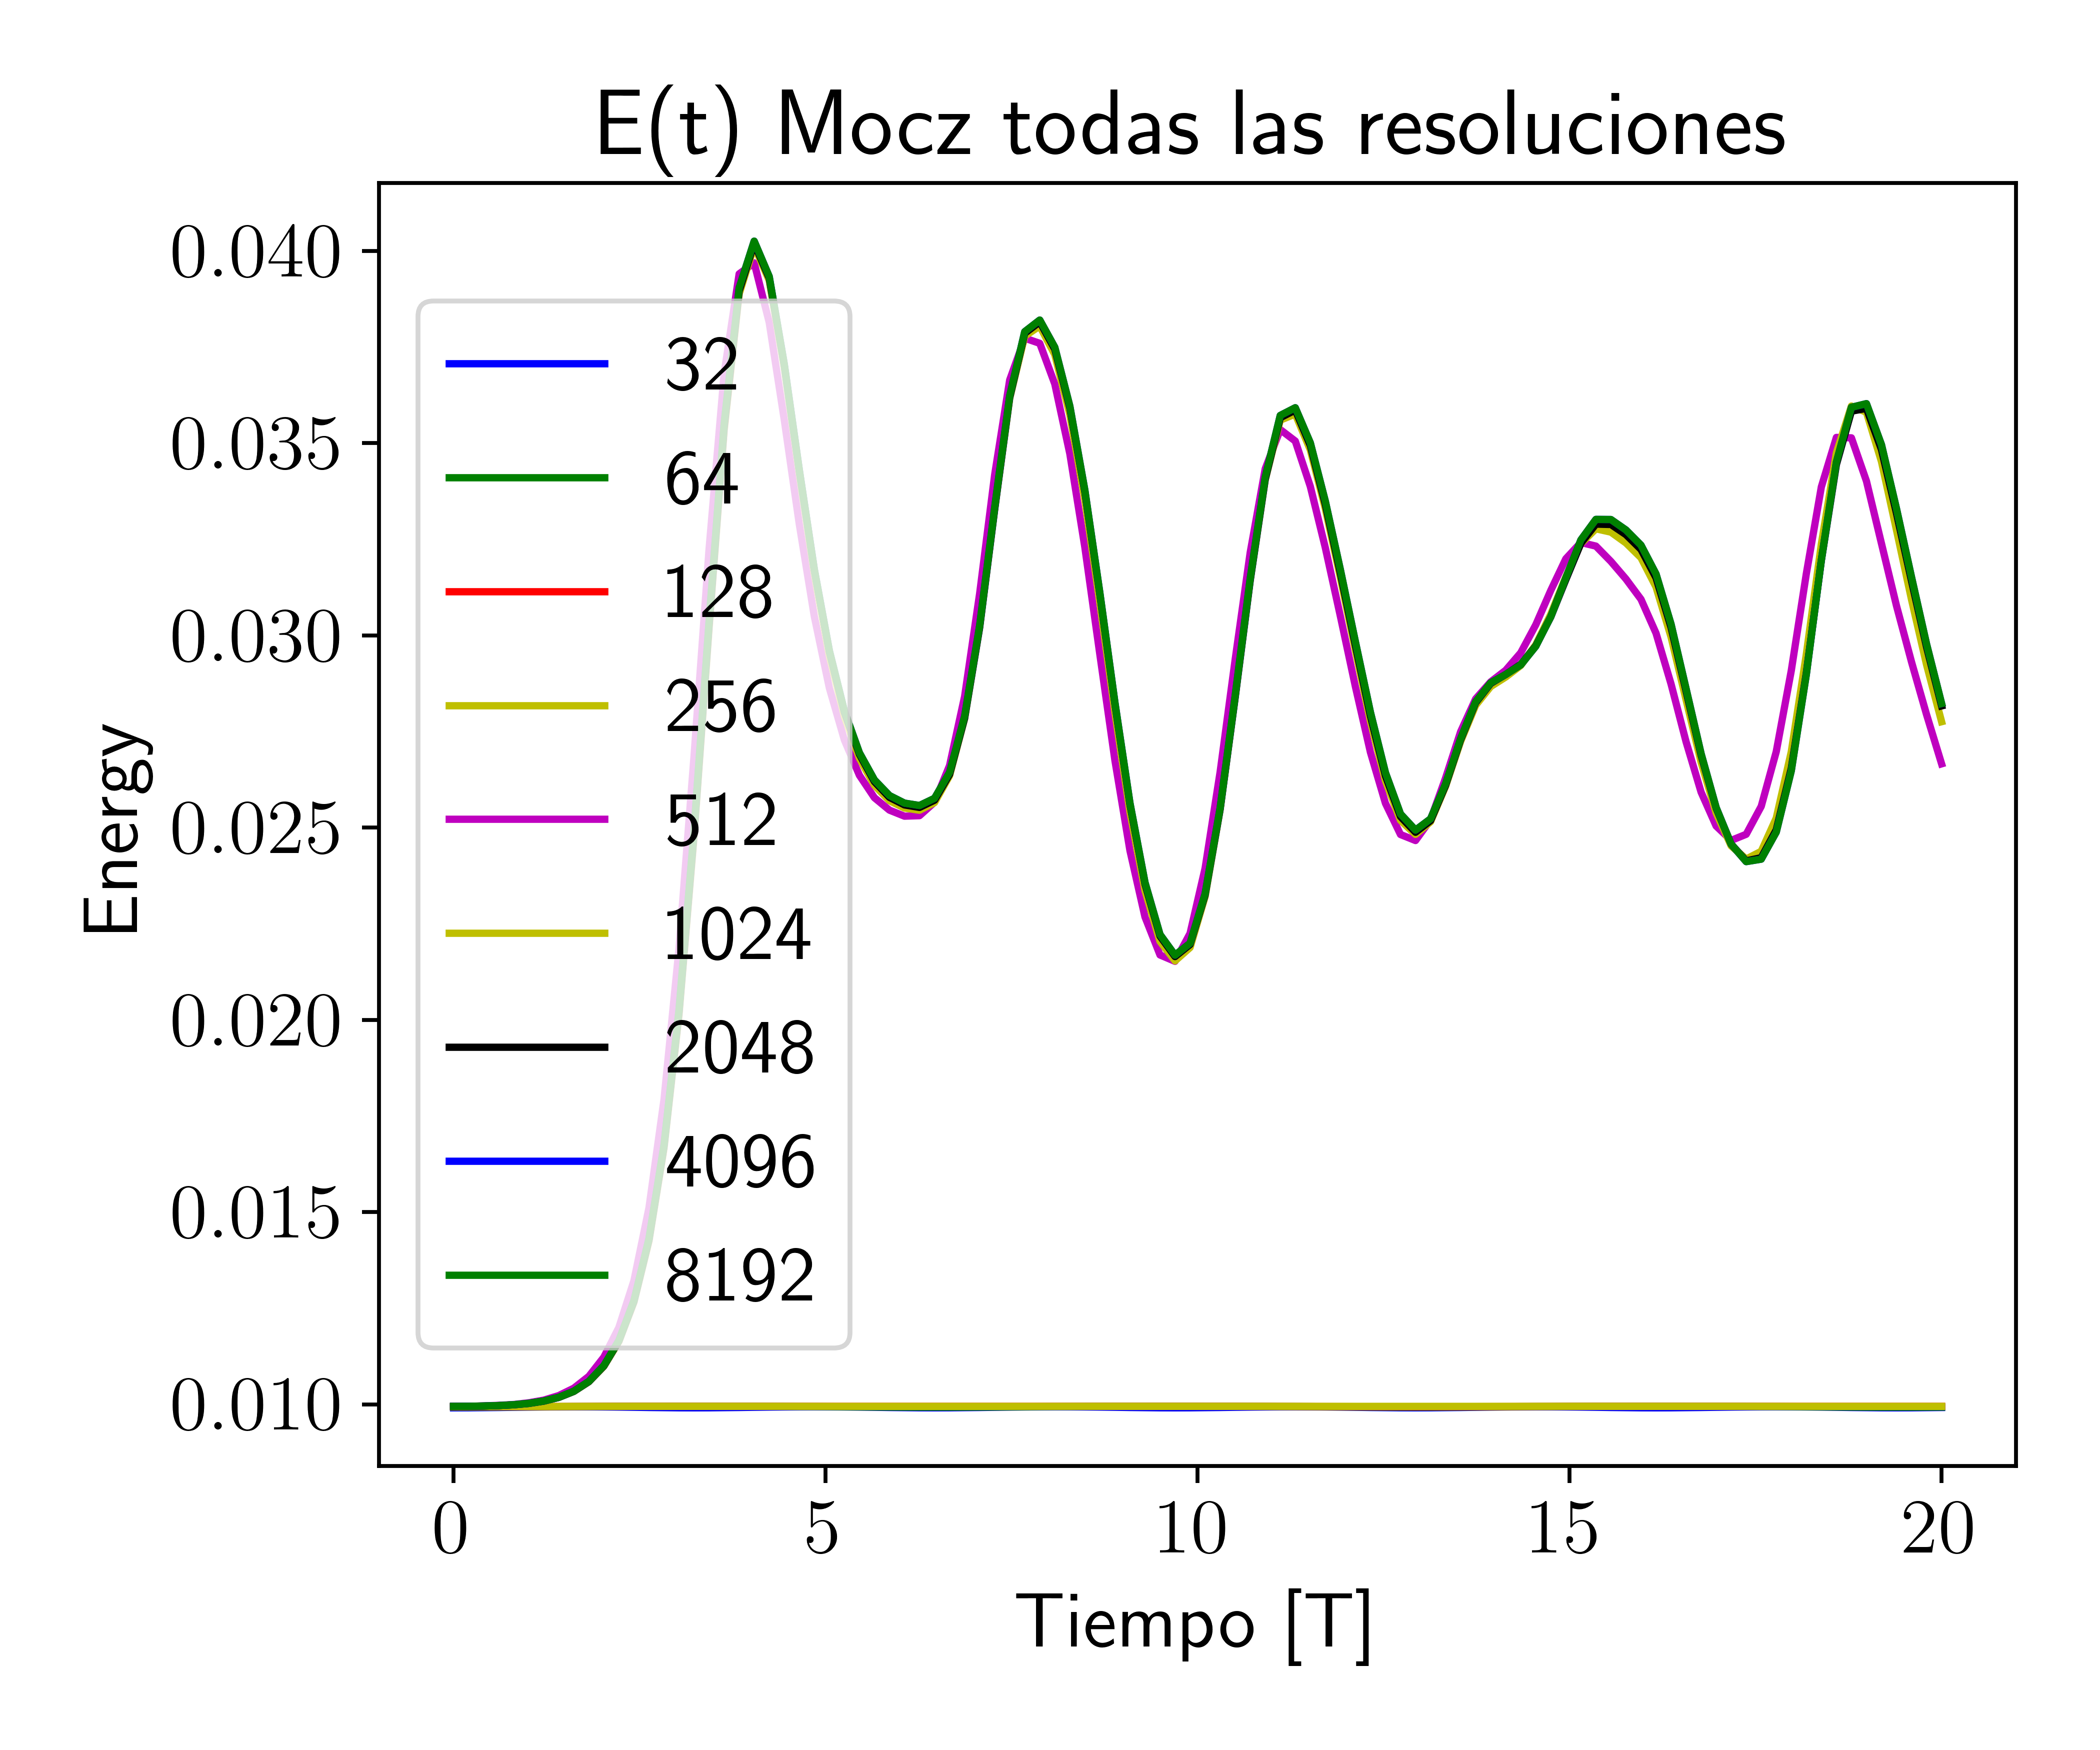
\includegraphics[scale= 0.6]{Jeans.png}
%  \caption{ asd}
  \label{fig: cobre}
\end{figure}	













                      
\bibliographystyle{unsrtnat} % estilo de las referencias 
\bibliography{bibTes.bib} %archivo con los datos de los artículos citados


%\bibliography{mybib.bib} %archivo con los datos de los artículos citados

% Forma Manual de hacer las referencias
% Se escribe todo a mano...
% Descomentar y jugar

%\begin{thebibliography}{99}
%\bibitem{Narasimhan1993}Narasimhan, M.N.L., (1993), \textit{Principles of
%Continuum Mechanics}, (John Willey, New York) p. 510.

%\bibitem{Demianski1985}Demia\'{n}ski M., (1985), \textit{Relativistic
%Astrophysics,} in International Series in Natural Philosophy, Vol 110, Edited
%by \textit{D. Ter Haar}, (Pergamon Press, Oxford).
%\end{thebibliography}
.
%Fin del documento
\end{document}


Así mismo, el factor de calidad $Q$ está dado por:
\begin{equation}
Q = \frac{1}{R} \sqrt\frac{L}{C}
\end{equation}
Por lo tanto, el valor del factor de calidad

%Todo lo que escriba aquí será ignorado, aunque no fuera un comentario...
\begin{table}[h!]
\centering
\begin{tabular}{|l|l|l|}
\hline
2 cm   & 4 cm   & 8 cm   \\ \hline
175,77 & 129,77 & 88,77  \\ \hline
223,77 & 129,77 & 114,77 \\ \hline
219,77 & 134,77 & 77,77  \\ \hline
190,77 & 120,77 & 83,77  \\ \hline
\end{tabular}
\caption{Número de colisiones a diferentes distancias en cinco minutos.}
\label{tiempoFijo}
\end{table}

\begin{figure}[h]
  \centering
   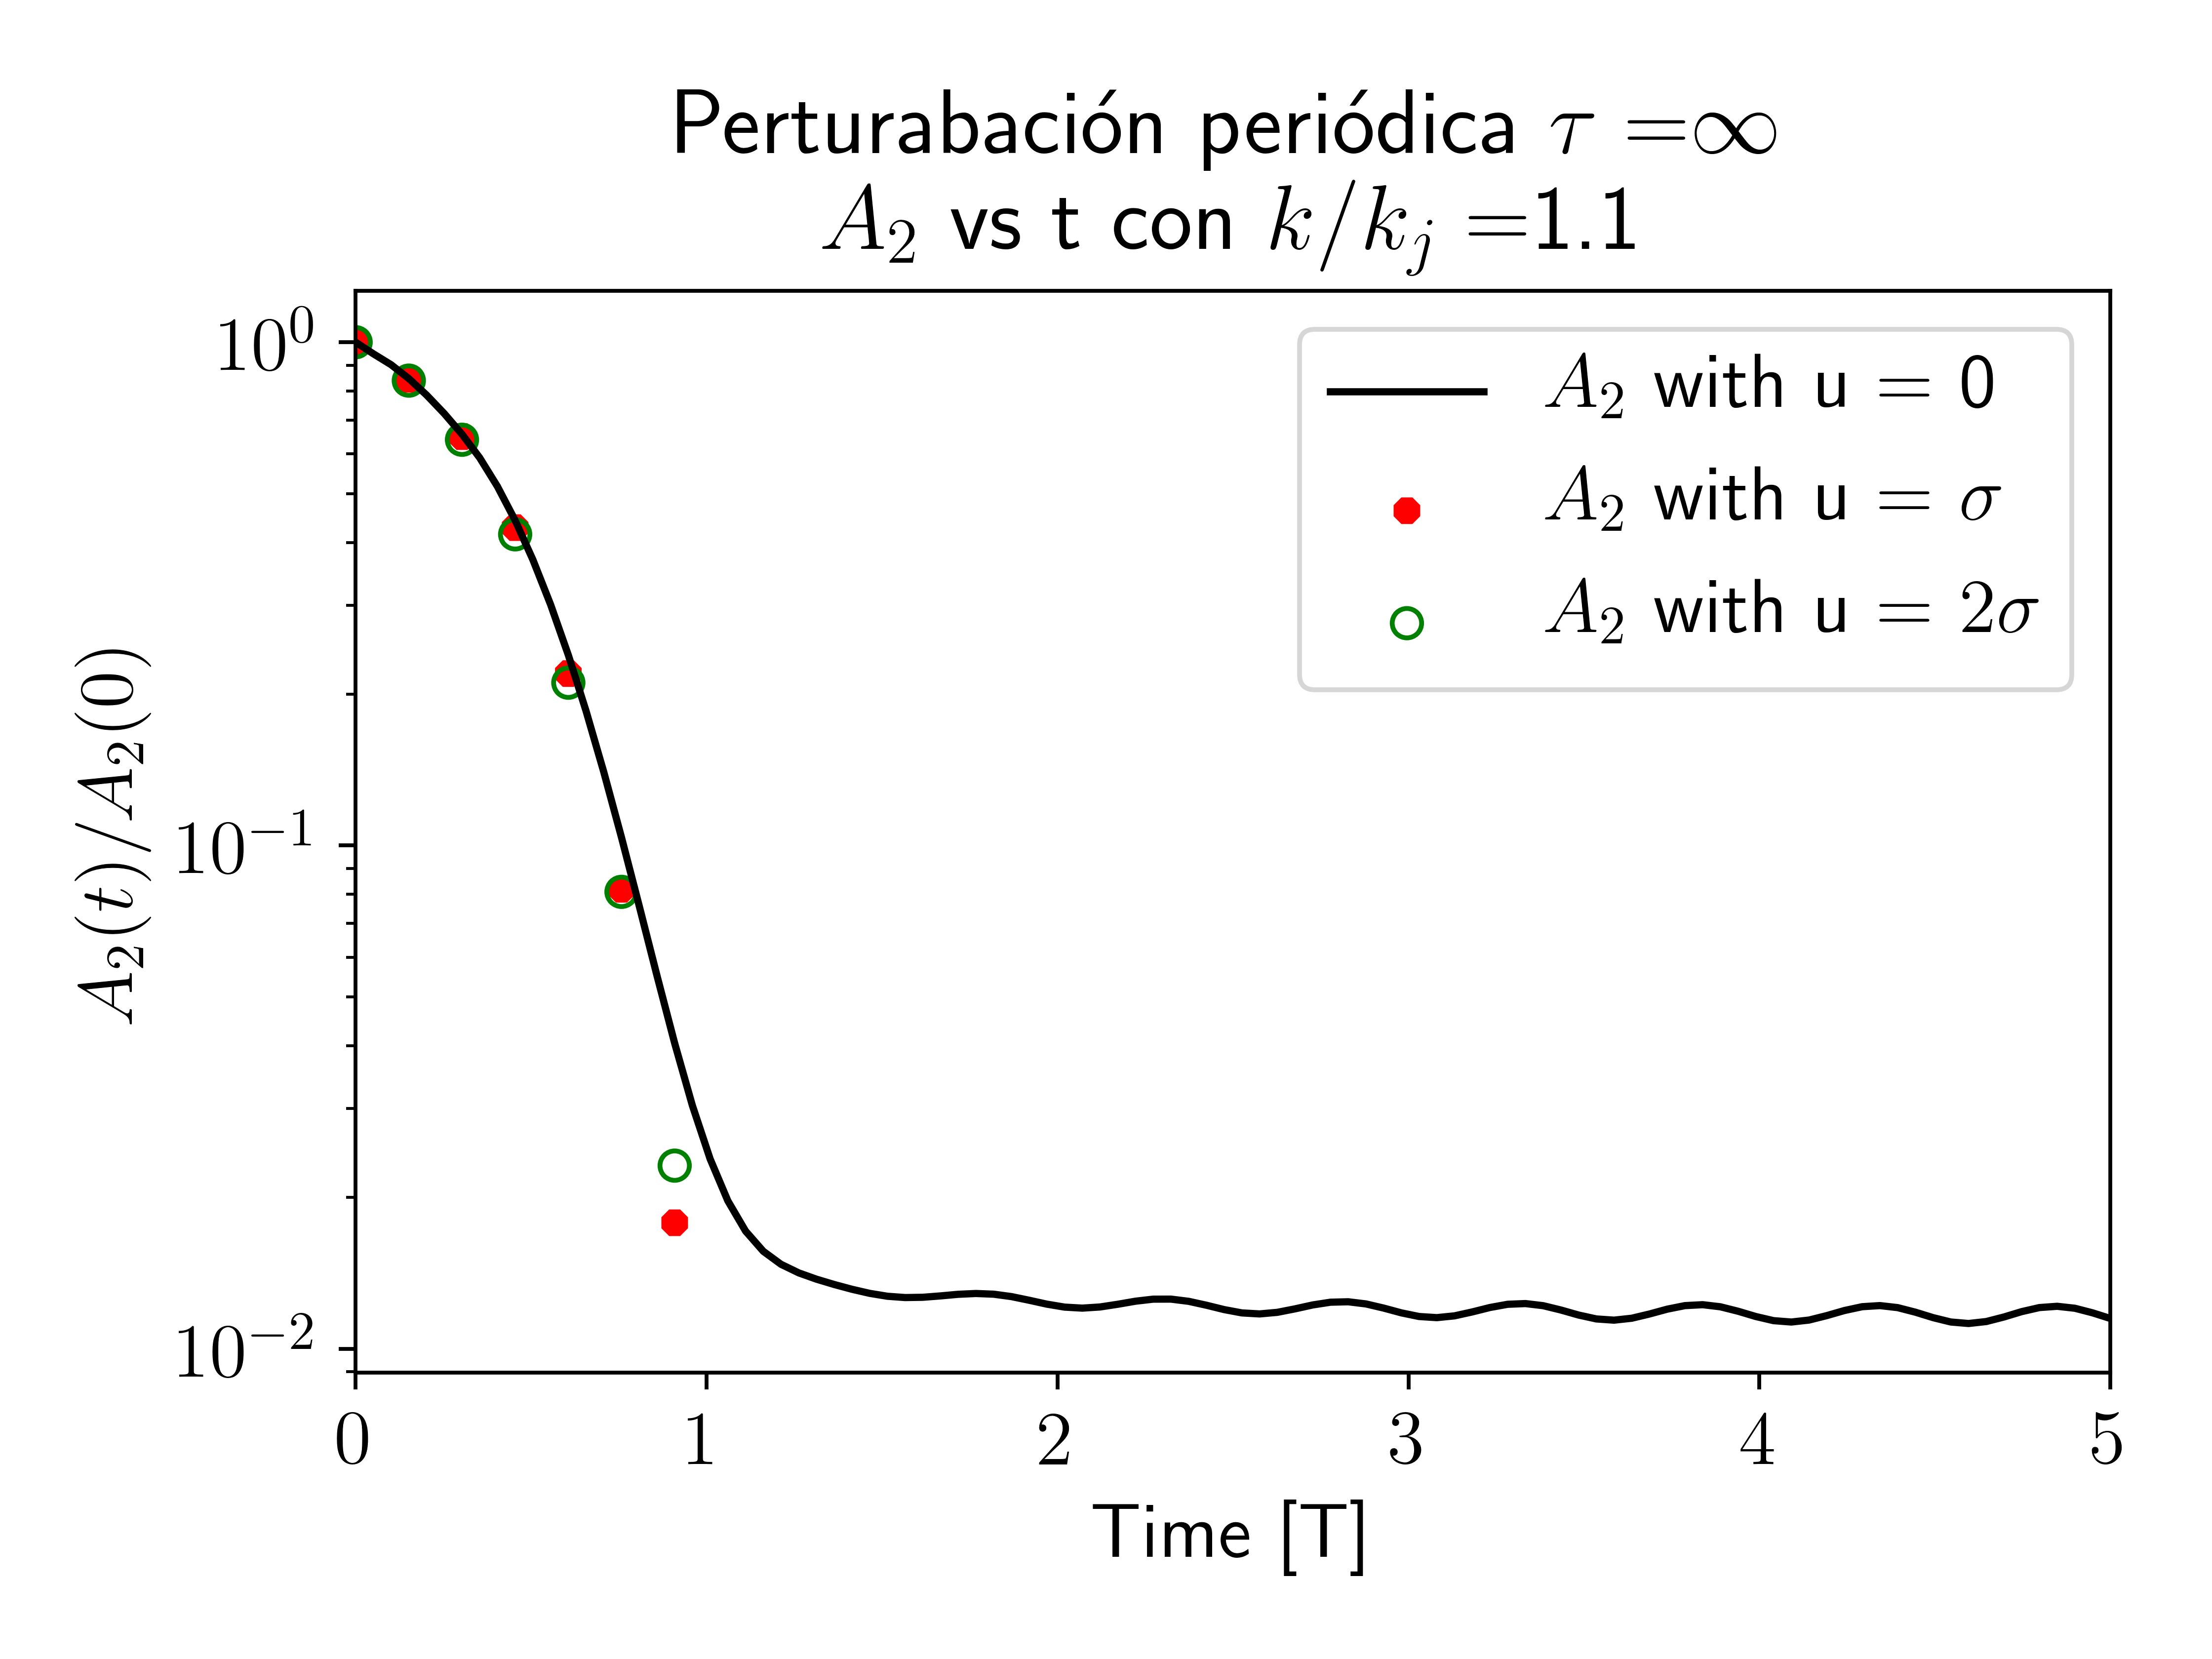
\includegraphics[scale= 0.8]{Jeans2Coef.png}

  \label{fig: cobre}
\end{figure}

\begin{figure}[h]
  \centering
   \includegraphics[scale= 0.8]{jairos.png}
  \caption{Gráfica del periodo de la pulsación para diferentes razones entre las frecuencias naturales utilizando una pesa de 200g. Es de resaltar que el pico no está centrado en 1 pero está bastante cerca. Esto probablemente se debe a errores a la hora de medir la longitud de los péndulos.}
  \label{fig: cobre}
\end{figure}
